% Options for packages loaded elsewhere
\PassOptionsToPackage{unicode}{hyperref}
\PassOptionsToPackage{hyphens}{url}
%
\documentclass[
]{article}
\usepackage{amsmath,amssymb}
\usepackage{iftex}
\ifPDFTeX
  \usepackage[T1]{fontenc}
  \usepackage[utf8]{inputenc}
  \usepackage{textcomp} % provide euro and other symbols
\else % if luatex or xetex
  \usepackage{unicode-math} % this also loads fontspec
  \defaultfontfeatures{Scale=MatchLowercase}
  \defaultfontfeatures[\rmfamily]{Ligatures=TeX,Scale=1}
\fi
\usepackage{lmodern}
\ifPDFTeX\else
  % xetex/luatex font selection
\fi
% Use upquote if available, for straight quotes in verbatim environments
\IfFileExists{upquote.sty}{\usepackage{upquote}}{}
\IfFileExists{microtype.sty}{% use microtype if available
  \usepackage[]{microtype}
  \UseMicrotypeSet[protrusion]{basicmath} % disable protrusion for tt fonts
}{}
\makeatletter
\@ifundefined{KOMAClassName}{% if non-KOMA class
  \IfFileExists{parskip.sty}{%
    \usepackage{parskip}
  }{% else
    \setlength{\parindent}{0pt}
    \setlength{\parskip}{6pt plus 2pt minus 1pt}}
}{% if KOMA class
  \KOMAoptions{parskip=half}}
\makeatother
\usepackage{xcolor}
\usepackage[margin=1in]{geometry}
\usepackage{color}
\usepackage{fancyvrb}
\newcommand{\VerbBar}{|}
\newcommand{\VERB}{\Verb[commandchars=\\\{\}]}
\DefineVerbatimEnvironment{Highlighting}{Verbatim}{commandchars=\\\{\}}
% Add ',fontsize=\small' for more characters per line
\usepackage{framed}
\definecolor{shadecolor}{RGB}{248,248,248}
\newenvironment{Shaded}{\begin{snugshade}}{\end{snugshade}}
\newcommand{\AlertTok}[1]{\textcolor[rgb]{0.94,0.16,0.16}{#1}}
\newcommand{\AnnotationTok}[1]{\textcolor[rgb]{0.56,0.35,0.01}{\textbf{\textit{#1}}}}
\newcommand{\AttributeTok}[1]{\textcolor[rgb]{0.13,0.29,0.53}{#1}}
\newcommand{\BaseNTok}[1]{\textcolor[rgb]{0.00,0.00,0.81}{#1}}
\newcommand{\BuiltInTok}[1]{#1}
\newcommand{\CharTok}[1]{\textcolor[rgb]{0.31,0.60,0.02}{#1}}
\newcommand{\CommentTok}[1]{\textcolor[rgb]{0.56,0.35,0.01}{\textit{#1}}}
\newcommand{\CommentVarTok}[1]{\textcolor[rgb]{0.56,0.35,0.01}{\textbf{\textit{#1}}}}
\newcommand{\ConstantTok}[1]{\textcolor[rgb]{0.56,0.35,0.01}{#1}}
\newcommand{\ControlFlowTok}[1]{\textcolor[rgb]{0.13,0.29,0.53}{\textbf{#1}}}
\newcommand{\DataTypeTok}[1]{\textcolor[rgb]{0.13,0.29,0.53}{#1}}
\newcommand{\DecValTok}[1]{\textcolor[rgb]{0.00,0.00,0.81}{#1}}
\newcommand{\DocumentationTok}[1]{\textcolor[rgb]{0.56,0.35,0.01}{\textbf{\textit{#1}}}}
\newcommand{\ErrorTok}[1]{\textcolor[rgb]{0.64,0.00,0.00}{\textbf{#1}}}
\newcommand{\ExtensionTok}[1]{#1}
\newcommand{\FloatTok}[1]{\textcolor[rgb]{0.00,0.00,0.81}{#1}}
\newcommand{\FunctionTok}[1]{\textcolor[rgb]{0.13,0.29,0.53}{\textbf{#1}}}
\newcommand{\ImportTok}[1]{#1}
\newcommand{\InformationTok}[1]{\textcolor[rgb]{0.56,0.35,0.01}{\textbf{\textit{#1}}}}
\newcommand{\KeywordTok}[1]{\textcolor[rgb]{0.13,0.29,0.53}{\textbf{#1}}}
\newcommand{\NormalTok}[1]{#1}
\newcommand{\OperatorTok}[1]{\textcolor[rgb]{0.81,0.36,0.00}{\textbf{#1}}}
\newcommand{\OtherTok}[1]{\textcolor[rgb]{0.56,0.35,0.01}{#1}}
\newcommand{\PreprocessorTok}[1]{\textcolor[rgb]{0.56,0.35,0.01}{\textit{#1}}}
\newcommand{\RegionMarkerTok}[1]{#1}
\newcommand{\SpecialCharTok}[1]{\textcolor[rgb]{0.81,0.36,0.00}{\textbf{#1}}}
\newcommand{\SpecialStringTok}[1]{\textcolor[rgb]{0.31,0.60,0.02}{#1}}
\newcommand{\StringTok}[1]{\textcolor[rgb]{0.31,0.60,0.02}{#1}}
\newcommand{\VariableTok}[1]{\textcolor[rgb]{0.00,0.00,0.00}{#1}}
\newcommand{\VerbatimStringTok}[1]{\textcolor[rgb]{0.31,0.60,0.02}{#1}}
\newcommand{\WarningTok}[1]{\textcolor[rgb]{0.56,0.35,0.01}{\textbf{\textit{#1}}}}
\usepackage{graphicx}
\makeatletter
\def\maxwidth{\ifdim\Gin@nat@width>\linewidth\linewidth\else\Gin@nat@width\fi}
\def\maxheight{\ifdim\Gin@nat@height>\textheight\textheight\else\Gin@nat@height\fi}
\makeatother
% Scale images if necessary, so that they will not overflow the page
% margins by default, and it is still possible to overwrite the defaults
% using explicit options in \includegraphics[width, height, ...]{}
\setkeys{Gin}{width=\maxwidth,height=\maxheight,keepaspectratio}
% Set default figure placement to htbp
\makeatletter
\def\fps@figure{htbp}
\makeatother
\setlength{\emergencystretch}{3em} % prevent overfull lines
\providecommand{\tightlist}{%
  \setlength{\itemsep}{0pt}\setlength{\parskip}{0pt}}
\setcounter{secnumdepth}{-\maxdimen} % remove section numbering
\ifLuaTeX
  \usepackage{selnolig}  % disable illegal ligatures
\fi
\IfFileExists{bookmark.sty}{\usepackage{bookmark}}{\usepackage{hyperref}}
\IfFileExists{xurl.sty}{\usepackage{xurl}}{} % add URL line breaks if available
\urlstyle{same}
\hypersetup{
  pdftitle={DEBY\_Raw\_Envr\_Data},
  hidelinks,
  pdfcreator={LaTeX via pandoc}}

\title{DEBY\_Raw\_Envr\_Data}
\author{}
\date{\vspace{-2.5em}2024-04-03}

\begin{document}
\maketitle

\begin{Shaded}
\begin{Highlighting}[]
\CommentTok{\#setwd("Users/madelineeppley/GitHub/MVP{-}H2F{-}HatcheryField/data/environment")}
\end{Highlighting}
\end{Shaded}

\hypertarget{load-required-packages.}{%
\subsubsection{Load required packages.}\label{load-required-packages.}}

\begin{Shaded}
\begin{Highlighting}[]
\FunctionTok{library}\NormalTok{(}\StringTok{"dplyr"}\NormalTok{) }\CommentTok{\#Used for working with data frames}
\end{Highlighting}
\end{Shaded}

\begin{verbatim}
## 
## Attaching package: 'dplyr'
\end{verbatim}

\begin{verbatim}
## The following objects are masked from 'package:stats':
## 
##     filter, lag
\end{verbatim}

\begin{verbatim}
## The following objects are masked from 'package:base':
## 
##     intersect, setdiff, setequal, union
\end{verbatim}

\begin{Shaded}
\begin{Highlighting}[]
\FunctionTok{library}\NormalTok{(}\StringTok{"lubridate"}\NormalTok{) }\CommentTok{\#Used for time{-}date conversions}
\end{Highlighting}
\end{Shaded}

\begin{verbatim}
## 
## Attaching package: 'lubridate'
\end{verbatim}

\begin{verbatim}
## The following objects are masked from 'package:base':
## 
##     date, intersect, setdiff, union
\end{verbatim}

\begin{Shaded}
\begin{Highlighting}[]
\FunctionTok{library}\NormalTok{(}\StringTok{"readr"}\NormalTok{) }\CommentTok{\#Used to read the CSV file}
\FunctionTok{library}\NormalTok{(}\StringTok{"ggplot2"}\NormalTok{) }
\end{Highlighting}
\end{Shaded}

\hypertarget{note-the-date-of-data-download-and-source.-all-available-data-should-be-used-for-each-site-regardless-of-year.-note-from-the-csv-file-how-often-the-site-was-sampled-and-if-there-are-replicates-in-the-data.-also-describe-if-the-sampling-occurred-at-only-low-tide-only-high-tide-or-continuously.}{%
\subsubsection{Note the date of data download and source. All available
data should be used for each site regardless of year. Note from the CSV
file how often the site was sampled, and if there are replicates in the
data. Also describe if the sampling occurred at only low tide, only high
tide, or
continuously.}\label{note-the-date-of-data-download-and-source.-all-available-data-should-be-used-for-each-site-regardless-of-year.-note-from-the-csv-file-how-often-the-site-was-sampled-and-if-there-are-replicates-in-the-data.-also-describe-if-the-sampling-occurred-at-only-low-tide-only-high-tide-or-continuously.}}

\begin{Shaded}
\begin{Highlighting}[]
\CommentTok{\#Data was downloaded on 04/02/2024}
\CommentTok{\#Source {-} http://vecos.vims.edu/StationDetail.aspx?param=YRK005.40\&program=CMON}
\CommentTok{\#The site was sampled continuously every 15 min from 2003}

\CommentTok{\#Create text strings with metadata information that we want to include in the final data frame. }
\NormalTok{download\_date }\OtherTok{\textless{}{-}}\NormalTok{ (}\StringTok{"04{-}02{-}2024"}\NormalTok{)}
\NormalTok{source\_description }\OtherTok{\textless{}{-}}\NormalTok{ (}\StringTok{"Virginia Estuarine and Coastal Observing System, VIMS"}\NormalTok{)}
\NormalTok{site\_name }\OtherTok{\textless{}{-}}\NormalTok{ (}\StringTok{"DEBY"}\NormalTok{) }
\NormalTok{collection\_type }\OtherTok{\textless{}{-}}\NormalTok{ (}\StringTok{"continuous"}\NormalTok{)}
\end{Highlighting}
\end{Shaded}

\hypertarget{use-the-file-path-name-in-your-working-directory-or-desktop-see-example-below.-or-import-data-set-through-the-files-window-in-r-studio.-store-the-file-in-a-variable-with-the-raw_id_site-format.-if-salinity-and-temperature-data-are-in-separate-files-read-in-both-and-store-them-with-_sal-or-_temp-in-the-variable-names.}{%
\subsubsection{Use the file path name in your working directory or
desktop, see example below. Or, import data set through the ``Files''
window in R studio. Store the file in a variable with the
``raw\_ID\_Site'' format. If salinity and temperature data are in
separate files, read in both and store them with ``\_sal'' or ``\_temp''
in the variable
names.}\label{use-the-file-path-name-in-your-working-directory-or-desktop-see-example-below.-or-import-data-set-through-the-files-window-in-r-studio.-store-the-file-in-a-variable-with-the-raw_id_site-format.-if-salinity-and-temperature-data-are-in-separate-files-read-in-both-and-store-them-with-_sal-or-_temp-in-the-variable-names.}}

\begin{Shaded}
\begin{Highlighting}[]
\CommentTok{\#The files we will be working with are from Gloucester Point, VA, which is for the DEBY selection line. The ID\_Site for this site is DEBY. }

\CommentTok{\#Environmental data could only be downloaded by year, so first we need to merge the yearly data sets.}
\NormalTok{data\_path }\OtherTok{\textless{}{-}} \StringTok{"/Users/madelineeppley/GitHub/MVP{-}H2F{-}HatcheryField/data/envr\_of\_origin/raw\_envr\_data/DEBY\_York\_raw\_yearly"}

\CommentTok{\# Read and merge all CSV files}
\NormalTok{raw\_DEBY\_env }\OtherTok{\textless{}{-}} \FunctionTok{list.files}\NormalTok{(}\AttributeTok{path =}\NormalTok{ data\_path, }\AttributeTok{full.names =} \ConstantTok{TRUE}\NormalTok{) }\SpecialCharTok{\%\textgreater{}\%}
  \FunctionTok{lapply}\NormalTok{(read.csv) }\SpecialCharTok{\%\textgreater{}\%}  \CommentTok{\# Use read\_csv from readr for better performance}
  \FunctionTok{bind\_rows}\NormalTok{()}


\CommentTok{\#The metadata for these data (located at the bottom of this site: http://vecos.vims.edu/Content.aspx?idContent=44) explain the various error codes listed alongside observations that are unusable or questionable. Error codes for a certain water quality observation are listed in a column titled WATERQUALITY\_A, where WATERQUALITY is whatever aspect of water quality is being measured. For example, next to the SALINITY column is SALINITY\_A, which lists error codes for salinity observations if applicable. Blank or NA WATERQUALITY\_A cells indicate no error code is applicable. We need to remove observations marked with these codes by keeping only data with blank cells or NA in these columns.}

\NormalTok{subset\_DEBY\_env\_error }\OtherTok{\textless{}{-}} \FunctionTok{subset}\NormalTok{(raw\_DEBY\_env, }\AttributeTok{select =} \FunctionTok{c}\NormalTok{(SAMPLE\_DATETIME, WTEMP, WTEMP\_A, SALINITY, SALINITY\_A)) }\CommentTok{\#subset data to include sample collection day and time, water temperature, water temperature error codes, salinity, and salinity error codes}

\NormalTok{subset1\_DEBY\_env }\OtherTok{\textless{}{-}}\NormalTok{ subset\_DEBY\_env\_error[(subset\_DEBY\_env\_error}\SpecialCharTok{$}\NormalTok{WTEMP\_A }\SpecialCharTok{\%in\%} \FunctionTok{c}\NormalTok{(}\StringTok{""}\NormalTok{, }\ConstantTok{NA}\NormalTok{)), ] }\CommentTok{\#keep only rows where the WTEMP\_A columns are blank or NA, i.e. where there were no error codes recorded for the temperature data, and save it to a new data frame}

\NormalTok{subset2\_DEBY\_env }\OtherTok{\textless{}{-}}\NormalTok{ subset1\_DEBY\_env[(subset1\_DEBY\_env}\SpecialCharTok{$}\NormalTok{SALINITY\_A }\SpecialCharTok{\%in\%} \FunctionTok{c}\NormalTok{(}\StringTok{""}\NormalTok{, }\ConstantTok{NA}\NormalTok{)),] }\CommentTok{\#keep only rows where the SALINITY\_A columns are blank or NA, i.e. where there were no error codes recorded for the salinity data, and save it to a new data frame}

\CommentTok{\# View(subset2\_DEBY\_env)}
\CommentTok{\#sorting the data frame by ascending and descending values for WTEMP\_A and SALINITY\_A shows only blank cells or NA for each of those columns. We have removed the data marked with error codes}

\NormalTok{subset\_DEBY\_env }\OtherTok{\textless{}{-}} \FunctionTok{subset}\NormalTok{(subset2\_DEBY\_env, }\AttributeTok{select =} \FunctionTok{c}\NormalTok{(SAMPLE\_DATETIME, WTEMP, SALINITY)) }\CommentTok{\#remove WTEMP\_A and SALINITY\_A from the dataframe now}

\CommentTok{\# View how the data are stored. Note the variable names and the format and units that the data are stored in.  }
\FunctionTok{summary}\NormalTok{(subset\_DEBY\_env)}
\end{Highlighting}
\end{Shaded}

\begin{verbatim}
##  SAMPLE_DATETIME        WTEMP           SALINITY    
##  Length:667345      Min.   : 0.020   Min.   : 8.06  
##  Class :character   1st Qu.: 9.639   1st Qu.:17.69  
##  Mode  :character   Median :17.300   Median :19.68  
##                     Mean   :17.122   Mean   :19.34  
##                     3rd Qu.:25.010   3rd Qu.:21.31  
##                     Max.   :32.290   Max.   :26.09
\end{verbatim}

\begin{Shaded}
\begin{Highlighting}[]
\CommentTok{\#rename columns. "datetime" = date and time of data collection, "temp" = water temperature in degrees C, "salinity" = water salinity in parts per thousand (ppt)}

\FunctionTok{colnames}\NormalTok{(subset\_DEBY\_env) }\OtherTok{\textless{}{-}} \FunctionTok{c}\NormalTok{(}\StringTok{"datetime"}\NormalTok{, }\StringTok{"temp"}\NormalTok{, }\StringTok{"salinity"}\NormalTok{)}
\end{Highlighting}
\end{Shaded}

\hypertarget{start-with-the-date-and-time-of-collection.-we-will-use-the-lubridate-package-to-standardize-all-values-into-the-date-time-format-called-posixct.-this-format-stores-the-date-and-time-in-number-of-seconds-since-a-past-point-111970.-this-makes-comparisons-easy-and-helps-to-standardizes-values.}{%
\subsubsection{Start with the date and time of collection. We will use
the lubridate package to standardize all values into the date-time
format called POSIXct. This format stores the date and time in number of
seconds since a past point (1/1/1970). This makes comparisons easy and
helps to standardizes
values.}\label{start-with-the-date-and-time-of-collection.-we-will-use-the-lubridate-package-to-standardize-all-values-into-the-date-time-format-called-posixct.-this-format-stores-the-date-and-time-in-number-of-seconds-since-a-past-point-111970.-this-makes-comparisons-easy-and-helps-to-standardizes-values.}}

\begin{Shaded}
\begin{Highlighting}[]
\CommentTok{\#Convert to POSIXct format. Tell R what the current date/time format is so it knows how to convert it. Store it into a column named datetime in the data frame.}
\NormalTok{subset\_DEBY\_env}\SpecialCharTok{$}\NormalTok{datetime }\OtherTok{\textless{}{-}} \FunctionTok{as.POSIXct}\NormalTok{(subset\_DEBY\_env}\SpecialCharTok{$}\NormalTok{datetime, }\StringTok{"\%m/\%d/\%Y \%H:\%M:\%S \%p"}\NormalTok{, }\AttributeTok{tz =} \StringTok{""}\NormalTok{)}


\CommentTok{\#Print the new data frame and examine to make sure the new datetime column is in the correct format. }
\FunctionTok{head}\NormalTok{(subset\_DEBY\_env)}
\end{Highlighting}
\end{Shaded}

\begin{verbatim}
##              datetime  temp salinity
## 1 2003-05-28 04:15:00 19.07    15.57
## 2 2003-05-28 04:30:00 19.15    15.45
## 3 2003-05-28 04:45:00 19.38    15.49
## 4 2003-05-28 05:00:00 19.81    15.58
## 5 2003-05-28 05:15:00 19.80    15.60
## 6 2003-05-28 05:30:00 19.89    15.56
\end{verbatim}

\hypertarget{standardize-column-and-variable-names.-we-will-use-lat-for-latitude-in-degrees-and-lon-for-longitude-in-degrees.}{%
\subsubsection{\#Standardize column and variable names. We will use
``lat'' for latitude in degrees, and ``lon'' for longitude in
degrees.}\label{standardize-column-and-variable-names.-we-will-use-lat-for-latitude-in-degrees-and-lon-for-longitude-in-degrees.}}

\begin{Shaded}
\begin{Highlighting}[]
\CommentTok{\#Store variables that we will include in the final data frame}
\NormalTok{lat }\OtherTok{\textless{}{-}} \FloatTok{37.247284}
\NormalTok{lon }\OtherTok{\textless{}{-}} \SpecialCharTok{{-}}\FloatTok{76.499369}
\NormalTok{firstyear }\OtherTok{\textless{}{-}} \DecValTok{2003}
\NormalTok{finalyear }\OtherTok{\textless{}{-}} \DecValTok{2024}
\end{Highlighting}
\end{Shaded}

\hypertarget{filter-any-of-the-variables-that-have-data-points-outside-of-normal-range.-we-will-use-0-40-as-the-accepted-range-for-salinity-ppt-and-temperature-c-values.-note-in-the-summer-salinity-values-can-sometimes-exceed-40.-check-to-see-if-there-are-values-above-40.-in-this-case-adjust-the-range-or-notify-someone-that-the-site-has-particularly-high-salinity-values.}{%
\subsubsection{Filter any of the variables that have data points outside
of normal range. We will use 0-40 as the accepted range for salinity
(ppt) and temperature (C) values. Note, in the summer, salinity values
can sometimes exceed 40. Check to see if there are values above 40. In
this case, adjust the range or notify someone that the site has
particularly high salinity
values.}\label{filter-any-of-the-variables-that-have-data-points-outside-of-normal-range.-we-will-use-0-40-as-the-accepted-range-for-salinity-ppt-and-temperature-c-values.-note-in-the-summer-salinity-values-can-sometimes-exceed-40.-check-to-see-if-there-are-values-above-40.-in-this-case-adjust-the-range-or-notify-someone-that-the-site-has-particularly-high-salinity-values.}}

\begin{Shaded}
\begin{Highlighting}[]
\CommentTok{\#Filter the data between the values of 0 and 40 for both salinity and temperature. }
\NormalTok{filtered\_DEBY\_sal }\OtherTok{\textless{}{-}}\NormalTok{ subset\_DEBY\_env }\SpecialCharTok{\%\textgreater{}\%}
    \FunctionTok{filter}\NormalTok{(}\FunctionTok{between}\NormalTok{(salinity, }\DecValTok{0}\NormalTok{, }\DecValTok{40}\NormalTok{)) }

\FunctionTok{summary}\NormalTok{(subset\_DEBY\_env)}
\end{Highlighting}
\end{Shaded}

\begin{verbatim}
##     datetime                           temp           salinity    
##  Min.   :2003-05-28 04:15:00.00   Min.   : 0.020   Min.   : 8.06  
##  1st Qu.:2008-12-20 09:30:00.00   1st Qu.: 9.639   1st Qu.:17.69  
##  Median :2014-01-13 02:30:00.00   Median :17.300   Median :19.68  
##  Mean   :2013-12-24 11:40:09.11   Mean   :17.122   Mean   :19.34  
##  3rd Qu.:2019-01-08 04:00:00.00   3rd Qu.:25.010   3rd Qu.:21.31  
##  Max.   :2024-01-11 12:45:00.00   Max.   :32.290   Max.   :26.09  
##  NA's   :152
\end{verbatim}

\begin{Shaded}
\begin{Highlighting}[]
\NormalTok{filtered\_DEBY\_env }\OtherTok{\textless{}{-}}\NormalTok{ filtered\_DEBY\_sal }\SpecialCharTok{\%\textgreater{}\%}
    \FunctionTok{filter}\NormalTok{(}\FunctionTok{between}\NormalTok{(temp, }\DecValTok{0}\NormalTok{, }\DecValTok{40}\NormalTok{))}

\CommentTok{\# Sanity check {-} print the ranges to ensure values are filtered properly. We can see that the ranges for both are now in the appropriate range.  }
\FunctionTok{print}\NormalTok{(}\FunctionTok{summary}\NormalTok{(filtered\_DEBY\_env}\SpecialCharTok{$}\NormalTok{salinity)) }
\end{Highlighting}
\end{Shaded}

\begin{verbatim}
##    Min. 1st Qu.  Median    Mean 3rd Qu.    Max. 
##    8.06   17.69   19.68   19.34   21.31   26.09
\end{verbatim}

\begin{Shaded}
\begin{Highlighting}[]
\FunctionTok{print}\NormalTok{(}\FunctionTok{summary}\NormalTok{(filtered\_DEBY\_env}\SpecialCharTok{$}\NormalTok{temp))}
\end{Highlighting}
\end{Shaded}

\begin{verbatim}
##    Min. 1st Qu.  Median    Mean 3rd Qu.    Max. 
##   0.020   9.639  17.300  17.122  25.010  32.290
\end{verbatim}

\begin{Shaded}
\begin{Highlighting}[]
\CommentTok{\#Store our data into a variable name with just the site name. }
\NormalTok{DEBY\_env }\OtherTok{\textless{}{-}}\NormalTok{ filtered\_DEBY\_env}

\CommentTok{\# we have NAs in the our data frame in the datetime column {-} need to remove these}
\NormalTok{count.nas\_env }\OtherTok{\textless{}{-}} \FunctionTok{is.na}\NormalTok{(DEBY\_env}\SpecialCharTok{$}\NormalTok{datetime) }\CommentTok{\# store our NAs in a variable}
\FunctionTok{summary}\NormalTok{(count.nas\_env) }\CommentTok{\# we have 152 NAs that are stored as "TRUE" in our count.nas}
\end{Highlighting}
\end{Shaded}

\begin{verbatim}
##    Mode   FALSE    TRUE 
## logical  667193     152
\end{verbatim}

\begin{Shaded}
\begin{Highlighting}[]
\FunctionTok{nrow}\NormalTok{(DEBY\_env) }\CommentTok{\# figure out how many rows we have in the original df: 667345}
\end{Highlighting}
\end{Shaded}

\begin{verbatim}
## [1] 667345
\end{verbatim}

\begin{Shaded}
\begin{Highlighting}[]
\FunctionTok{which}\NormalTok{(count.nas\_env }\SpecialCharTok{==} \ConstantTok{TRUE}\NormalTok{) }\CommentTok{\# find the number of NA rows that we need to remove: 152}
\end{Highlighting}
\end{Shaded}

\begin{verbatim}
##   [1]  19905  19906  19907  19908  19953  19954  19955  19956  46203  46204
##  [11]  46205  46206  46251  46252  46253  46254  79678  79679  79680  79681
##  [21]  79726  79727  79728  79729 108089 108090 108091 108092 108137 108138
##  [31] 108139 108140 141594 141595 141596 141597 141642 141643 141644 141645
##  [41] 174170 174171 174172 174173 174218 174219 174220 174221 206883 206884
##  [51] 206885 206886 206931 206932 206933 206934 237216 237217 237218 237219
##  [61] 237264 237265 237266 237267 271307 271308 271309 271310 271355 271356
##  [71] 271357 271358 305058 305059 305060 305061 305106 305107 305108 305109
##  [81] 338850 338851 338852 338853 338898 338899 338900 338901 372369 372370
##  [91] 372371 372372 372417 372418 372419 372420 405987 405988 405989 405990
## [101] 406035 406036 406037 406038 439794 439795 439796 439797 439842 439843
## [111] 439844 439845 472348 472349 472350 472351 472396 472397 472398 472399
## [121] 506313 506314 506315 506316 506358 506359 506360 506361 539401 539402
## [131] 539403 539404 539449 539450 539451 539452 605533 605534 605535 605536
## [141] 605581 605582 605583 605584 640317 640318 640319 640320 640365 640366
## [151] 640367 640368
\end{verbatim}

\begin{Shaded}
\begin{Highlighting}[]
\NormalTok{DEBY\_env }\OtherTok{\textless{}{-}} \FunctionTok{na.omit}\NormalTok{(DEBY\_env) }\CommentTok{\#remove NAs using na.omit}
\FunctionTok{nrow}\NormalTok{(DEBY\_env) }\CommentTok{\#there are 667193 rows in the new data frame}
\end{Highlighting}
\end{Shaded}

\begin{verbatim}
## [1] 667193
\end{verbatim}

\begin{Shaded}
\begin{Highlighting}[]
\NormalTok{check\_env }\OtherTok{\textless{}{-}} \DecValTok{667345} \SpecialCharTok{{-}} \DecValTok{667193}\CommentTok{\#the value of the check should be 152}
\NormalTok{check\_env }\CommentTok{\#we removed 152 NA rows!}
\end{Highlighting}
\end{Shaded}

\begin{verbatim}
## [1] 152
\end{verbatim}

\begin{Shaded}
\begin{Highlighting}[]
\CommentTok{\# check for NAs in our temperature column}
\NormalTok{count.nas\_temp }\OtherTok{\textless{}{-}} \FunctionTok{is.na}\NormalTok{(DEBY\_env}\SpecialCharTok{$}\NormalTok{temp) }\CommentTok{\# store our NAs in temp in a variable}
\FunctionTok{summary}\NormalTok{(count.nas\_temp) }\CommentTok{\# we have 0 NAs}
\end{Highlighting}
\end{Shaded}

\begin{verbatim}
##    Mode   FALSE 
## logical  667193
\end{verbatim}

\begin{Shaded}
\begin{Highlighting}[]
\CommentTok{\#check for NAs in our temperature column}
\NormalTok{count.nas\_sal }\OtherTok{\textless{}{-}} \FunctionTok{is.na}\NormalTok{(DEBY\_env}\SpecialCharTok{$}\NormalTok{salinity) }\CommentTok{\#store our NAs in salinity in a variable}
\FunctionTok{summary}\NormalTok{(count.nas\_sal) }\CommentTok{\#we have no NAs}
\end{Highlighting}
\end{Shaded}

\begin{verbatim}
##    Mode   FALSE 
## logical  667193
\end{verbatim}

\#Data sets for violin plots

\begin{Shaded}
\begin{Highlighting}[]
\CommentTok{\#add site name and create new data frame with full envr data set}
\NormalTok{DEBY\_env\_full }\OtherTok{\textless{}{-}}\NormalTok{ DEBY\_env }\SpecialCharTok{\%\textgreater{}\%} 
  \FunctionTok{mutate}\NormalTok{(site\_name, }\AttributeTok{site\_name =} \StringTok{"DEBY"}\NormalTok{)}

\CommentTok{\#reorder columns with site\_name first}
\NormalTok{DEBY\_env\_full }\OtherTok{\textless{}{-}}\NormalTok{ DEBY\_env\_full[, }\FunctionTok{c}\NormalTok{(}\DecValTok{4}\NormalTok{, }\DecValTok{1}\NormalTok{, }\DecValTok{2}\NormalTok{, }\DecValTok{3}\NormalTok{)]}

\NormalTok{DEBY\_temp\_full }\OtherTok{\textless{}{-}}\NormalTok{ DEBY\_env\_full[, }\FunctionTok{c}\NormalTok{(}\DecValTok{1}\NormalTok{,}\DecValTok{2}\NormalTok{,}\DecValTok{3}\NormalTok{)]}

\NormalTok{DEBY\_sal\_full }\OtherTok{\textless{}{-}}\NormalTok{ DEBY\_env\_full[, }\FunctionTok{c}\NormalTok{(}\DecValTok{1}\NormalTok{, }\DecValTok{2}\NormalTok{, }\DecValTok{4}\NormalTok{)]}

\CommentTok{\#save DEBY\_temp\_full and DEBY\_sal\_full as csv files for future analyses}
\FunctionTok{write.csv}\NormalTok{(DEBY\_temp\_full, }\StringTok{"../../data/envr\_of\_origin/full\_temp/DEBY\_temp\_full.csv"}\NormalTok{, }\AttributeTok{row.names =} \ConstantTok{FALSE}\NormalTok{)}
\FunctionTok{write.csv}\NormalTok{(DEBY\_sal\_full, }\StringTok{"../../data/envr\_of\_origin/full\_sal/DEBY\_sal\_full.csv"}\NormalTok{, }\AttributeTok{row.names =} \ConstantTok{FALSE}\NormalTok{)}
\end{Highlighting}
\end{Shaded}

\hypertarget{visualize-the-salinity-temperature-and-date-ranges-over-time.-this-can-help-us-see-if-there-are-any-anomalies-or-gaps-in-the-data-and-make-sure-the-filtering-was-done-correctly.-sanity-check---do-the-temperature-and-salinity-ranges-look-appropriate-for-the-geography-of-the-site-ex.-near-full-ocean-salinity-for-coastal-sites-lower-salinity-for-estuaries-or-near-rivers}{%
\subsubsection{Visualize the salinity, temperature, and date ranges over
time. This can help us see if there are any anomalies or gaps in the
data and make sure the filtering was done correctly. Sanity check - do
the temperature and salinity ranges look appropriate for the geography
of the site (ex. near full ocean salinity for coastal sites, lower
salinity for estuaries or near
rivers)?}\label{visualize-the-salinity-temperature-and-date-ranges-over-time.-this-can-help-us-see-if-there-are-any-anomalies-or-gaps-in-the-data-and-make-sure-the-filtering-was-done-correctly.-sanity-check---do-the-temperature-and-salinity-ranges-look-appropriate-for-the-geography-of-the-site-ex.-near-full-ocean-salinity-for-coastal-sites-lower-salinity-for-estuaries-or-near-rivers}}

\begin{Shaded}
\begin{Highlighting}[]
\NormalTok{salplot }\OtherTok{\textless{}{-}} \FunctionTok{ggplot}\NormalTok{(DEBY\_env, }\FunctionTok{aes}\NormalTok{(}\AttributeTok{x =}\NormalTok{ datetime)) }\SpecialCharTok{+}
    \FunctionTok{geom\_line}\NormalTok{(}\FunctionTok{aes}\NormalTok{(}\AttributeTok{y =}\NormalTok{ salinity, }\AttributeTok{color =} \StringTok{"Salinity (ppt)"}\NormalTok{)) }\SpecialCharTok{+}
    \FunctionTok{ylim}\NormalTok{(}\DecValTok{0}\NormalTok{,}\DecValTok{40}\NormalTok{) }\SpecialCharTok{+}
    \FunctionTok{labs}\NormalTok{(}\AttributeTok{x =} \StringTok{"Time"}\NormalTok{, }\AttributeTok{y =} \StringTok{"Salinity ppt"}\NormalTok{, }\AttributeTok{title =} \StringTok{"Salinity Plot for DEBY {-} Gloucester Point, Virginia"}\NormalTok{) }\SpecialCharTok{+}
    \FunctionTok{scale\_color\_manual}\NormalTok{(}\AttributeTok{values =} \FunctionTok{c}\NormalTok{(}\StringTok{"Salinity (ppt)"} \OtherTok{=} \StringTok{"blue"}\NormalTok{)) }\SpecialCharTok{+}
    \FunctionTok{theme\_minimal}\NormalTok{()}


\NormalTok{salplot}
\end{Highlighting}
\end{Shaded}

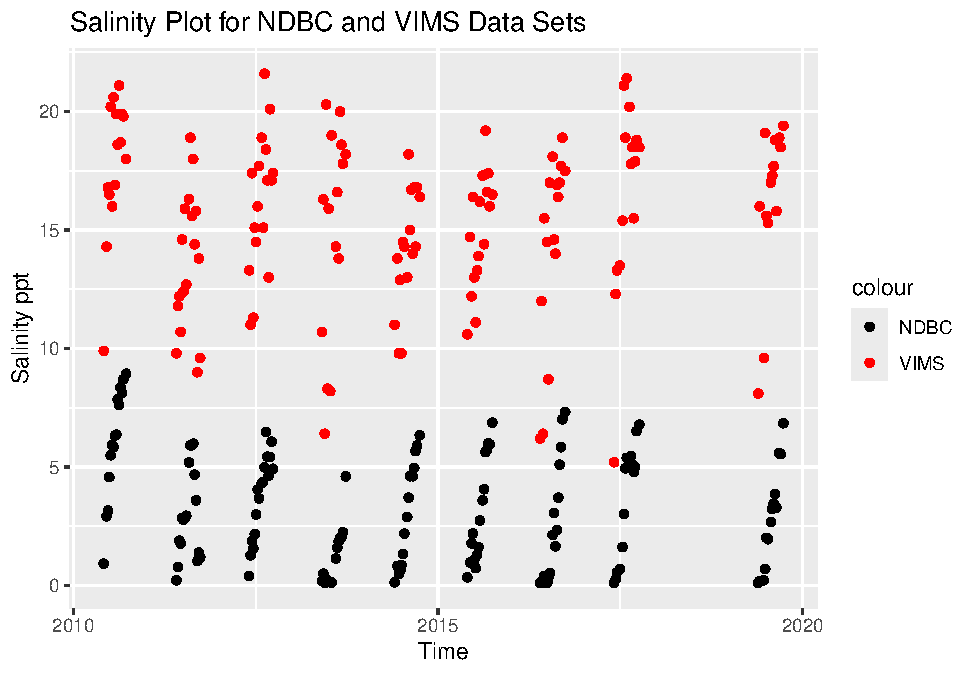
\includegraphics{DEBY_raw_env_files/figure-latex/salinity-plot-1.pdf}

\begin{Shaded}
\begin{Highlighting}[]
\NormalTok{tempplot }\OtherTok{\textless{}{-}} \FunctionTok{ggplot}\NormalTok{(DEBY\_env, }\FunctionTok{aes}\NormalTok{(}\AttributeTok{x =}\NormalTok{ datetime)) }\SpecialCharTok{+}
    \FunctionTok{geom\_line}\NormalTok{(}\FunctionTok{aes}\NormalTok{(}\AttributeTok{y =}\NormalTok{ temp, }\AttributeTok{color =} \StringTok{"Temperature (C)"}\NormalTok{)) }\SpecialCharTok{+}
    \FunctionTok{ylim}\NormalTok{(}\DecValTok{0}\NormalTok{, }\DecValTok{40}\NormalTok{) }\SpecialCharTok{+}
    \FunctionTok{labs}\NormalTok{(}\AttributeTok{x =} \StringTok{"Time"}\NormalTok{, }\AttributeTok{y =} \StringTok{"Temperature C"}\NormalTok{, }\AttributeTok{title =} \StringTok{"Temperature Plot for DEBY {-} Gloucester Point, Virginia"}\NormalTok{) }\SpecialCharTok{+}
    \FunctionTok{scale\_color\_manual}\NormalTok{(}\AttributeTok{values =} \FunctionTok{c}\NormalTok{( }\StringTok{"Temperature (C)"} \OtherTok{=} \StringTok{"red"}\NormalTok{)) }\SpecialCharTok{+}
    \FunctionTok{theme\_minimal}\NormalTok{()}

\NormalTok{tempplot}
\end{Highlighting}
\end{Shaded}

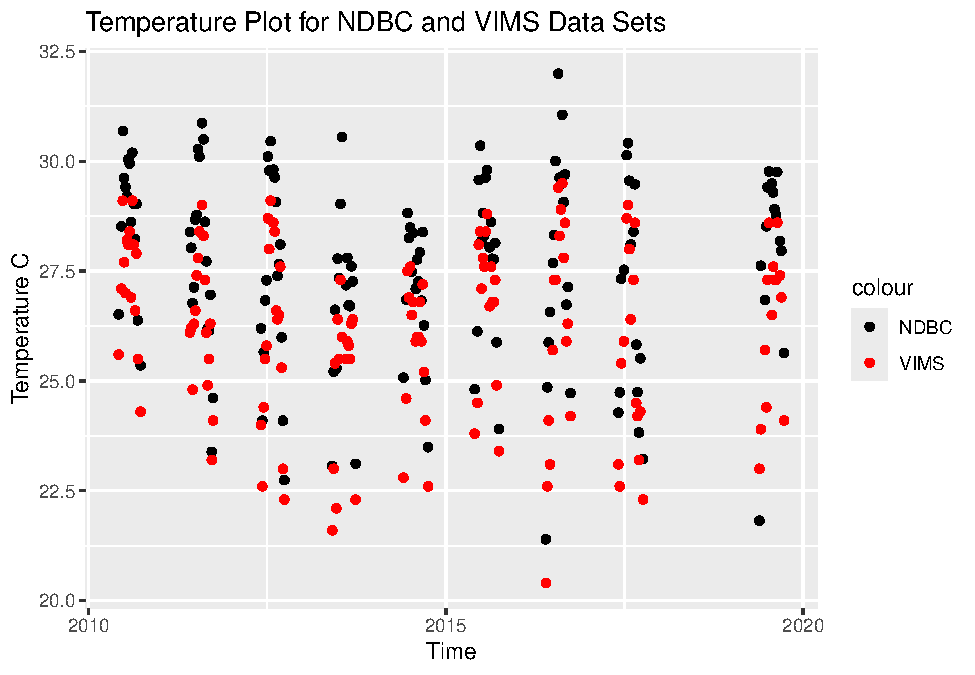
\includegraphics{DEBY_raw_env_files/figure-latex/temperature-plot-1.pdf}

\hypertarget{we-need-to-calculate-the-mean-maximum-and-minimum-values-for-salinity-and-temperature-per-month-and-year.-first-make-two-data-frames-to-contain-each-of-the-annual-and-monthly-averages.}{%
\subsubsection{We need to calculate the mean, maximum, and minimum
values for salinity and temperature per month and year. First make two
data frames to contain each of the annual and monthly
averages.}\label{we-need-to-calculate-the-mean-maximum-and-minimum-values-for-salinity-and-temperature-per-month-and-year.-first-make-two-data-frames-to-contain-each-of-the-annual-and-monthly-averages.}}

\begin{Shaded}
\begin{Highlighting}[]
\NormalTok{S2\_DEBY }\OtherTok{\textless{}{-}}\NormalTok{ DEBY\_env}

\CommentTok{\#Calculate the mean, maximum, and minimum values for salinity and temperature for each month. }
\NormalTok{S2\_DEBY\_envrmonth }\OtherTok{\textless{}{-}}\NormalTok{ S2\_DEBY }\SpecialCharTok{\%\textgreater{}\%}
    \FunctionTok{mutate}\NormalTok{(}\AttributeTok{year =} \FunctionTok{year}\NormalTok{(datetime), }\AttributeTok{month =} \FunctionTok{month}\NormalTok{(datetime)) }\SpecialCharTok{\%\textgreater{}\%}
    \FunctionTok{group\_by}\NormalTok{(year, month) }\SpecialCharTok{\%\textgreater{}\%}
    \FunctionTok{summarise}\NormalTok{(}
      \AttributeTok{min\_salinity =} \FunctionTok{min}\NormalTok{(salinity),}
      \AttributeTok{max\_salinity =} \FunctionTok{max}\NormalTok{(salinity),}
      \AttributeTok{mean\_salinity =} \FunctionTok{mean}\NormalTok{(salinity),}
      \AttributeTok{length\_salinity =} \FunctionTok{length}\NormalTok{(salinity),}
      \AttributeTok{min\_temp =} \FunctionTok{min}\NormalTok{(temp),}
      \AttributeTok{max\_temp =} \FunctionTok{max}\NormalTok{(temp),}
      \AttributeTok{mean\_temp =} \FunctionTok{mean}\NormalTok{(temp),}
      \AttributeTok{length\_temp =} \FunctionTok{length}\NormalTok{(temp))}
\end{Highlighting}
\end{Shaded}

\begin{verbatim}
## `summarise()` has grouped output by 'year'. You can override using the
## `.groups` argument.
\end{verbatim}

\begin{Shaded}
\begin{Highlighting}[]
\FunctionTok{print}\NormalTok{(S2\_DEBY\_envrmonth)}
\end{Highlighting}
\end{Shaded}

\begin{verbatim}
## # A tibble: 246 x 10
## # Groups:   year [22]
##     year month min_salinity max_salinity mean_salinity length_salinity min_temp
##    <dbl> <dbl>        <dbl>        <dbl>         <dbl>           <int>    <dbl>
##  1  2003     5         12.7         15.7          14.4             319    18.6 
##  2  2003     6         11.9         19.3          14.7            2880    17.1 
##  3  2003     7         14.3         21.9          18.0            2976    23.7 
##  4  2003     8         14.3         20.6          18.1            2976    25.0 
##  5  2003     9         13.0         21.4          17.4            2880    21.7 
##  6  2003    10         12.2         19.7          16.4            2975    15.4 
##  7  2003    11         13.2         20.4          16.8            2880     9.61
##  8  2003    12         14.4         16.2          15.5              33    10.4 
##  9  2004     2         12.2         15.5          14.1             241     4.5 
## 10  2004     3         13.0         19.7          16.4            1448     5.27
## # i 236 more rows
## # i 3 more variables: max_temp <dbl>, mean_temp <dbl>, length_temp <int>
\end{verbatim}

\begin{Shaded}
\begin{Highlighting}[]
\CommentTok{\#Calculate the mean, maximum, and minimum values for salinity and temperature for each year. }
\NormalTok{S2\_DEBY\_envryear }\OtherTok{\textless{}{-}}\NormalTok{ S2\_DEBY }\SpecialCharTok{\%\textgreater{}\%}
    \FunctionTok{mutate}\NormalTok{(}\AttributeTok{year =} \FunctionTok{year}\NormalTok{(datetime)) }\SpecialCharTok{\%\textgreater{}\%}
    \FunctionTok{group\_by}\NormalTok{(year) }\SpecialCharTok{\%\textgreater{}\%}
    \FunctionTok{summarise}\NormalTok{(}
      \AttributeTok{min\_salinity =} \FunctionTok{min}\NormalTok{(salinity),}
      \AttributeTok{max\_salinity =} \FunctionTok{max}\NormalTok{(salinity),}
      \AttributeTok{mean\_salinity =} \FunctionTok{mean}\NormalTok{(salinity),}
      \AttributeTok{min\_temp =} \FunctionTok{min}\NormalTok{(temp),}
      \AttributeTok{max\_temp =} \FunctionTok{max}\NormalTok{(temp),}
      \AttributeTok{mean\_temp =} \FunctionTok{mean}\NormalTok{(temp))}

\FunctionTok{print}\NormalTok{(S2\_DEBY\_envryear)}
\end{Highlighting}
\end{Shaded}

\begin{verbatim}
## # A tibble: 22 x 7
##     year min_salinity max_salinity mean_salinity min_temp max_temp mean_temp
##    <dbl>        <dbl>        <dbl>         <dbl>    <dbl>    <dbl>     <dbl>
##  1  2003        11.9          21.9          16.9     9.61     30.3      22.4
##  2  2004        10.5          22.4          17.2     4.5      30.1      20.6
##  3  2005         9.68         23.7          18.6     4.05     31.9      18.4
##  4  2006        13.8          23.6          19.1     4.97     32.3      16.0
##  5  2007        11.9          24.6          20.1     2.02     32.2      17.1
##  6  2008        13.2          24.4          20.1     3.92     31.7      16.4
##  7  2009        11.9          22.6          19.8     2.09     30.1      15.9
##  8  2010        11.2          25.4          20.1     1.01     30.8      16.0
##  9  2011        11.4          23.6          18.1     1.02     32.0      16.9
## 10  2012        14.1          24.5          19.7     5.86     30.8      17.5
## # i 12 more rows
\end{verbatim}

\begin{Shaded}
\begin{Highlighting}[]
\CommentTok{\#Calculate the mean, maximum, and minimum values for salinity and temperature for each day. }
\NormalTok{S2\_DEBY\_envrday }\OtherTok{\textless{}{-}}\NormalTok{ S2\_DEBY }\SpecialCharTok{\%\textgreater{}\%}
    \FunctionTok{mutate}\NormalTok{(}\AttributeTok{year =} \FunctionTok{year}\NormalTok{(datetime), }\AttributeTok{month =} \FunctionTok{month}\NormalTok{(datetime), }\AttributeTok{day =} \FunctionTok{day}\NormalTok{(datetime)) }\SpecialCharTok{\%\textgreater{}\%}
    \FunctionTok{group\_by}\NormalTok{(year, month, day) }\SpecialCharTok{\%\textgreater{}\%}
    \FunctionTok{summarise}\NormalTok{(}
      \AttributeTok{min\_salinity =} \FunctionTok{min}\NormalTok{(salinity),}
      \AttributeTok{max\_salinity =} \FunctionTok{max}\NormalTok{(salinity),}
      \AttributeTok{mean\_salinity =} \FunctionTok{mean}\NormalTok{(salinity),}
      \AttributeTok{length\_salinity =} \FunctionTok{length}\NormalTok{(salinity),}
      \AttributeTok{min\_temp =} \FunctionTok{min}\NormalTok{(temp),}
      \AttributeTok{max\_temp =} \FunctionTok{max}\NormalTok{(temp),}
      \AttributeTok{mean\_temp =} \FunctionTok{mean}\NormalTok{(temp),}
      \AttributeTok{length\_temp =} \FunctionTok{length}\NormalTok{(temp))}
\end{Highlighting}
\end{Shaded}

\begin{verbatim}
## `summarise()` has grouped output by 'year', 'month'. You can override using the
## `.groups` argument.
\end{verbatim}

\begin{Shaded}
\begin{Highlighting}[]
\FunctionTok{print}\NormalTok{(S2\_DEBY\_envrday)}
\end{Highlighting}
\end{Shaded}

\begin{verbatim}
## # A tibble: 7,079 x 11
## # Groups:   year, month [246]
##     year month   day min_salinity max_salinity mean_salinity length_salinity
##    <dbl> <dbl> <int>        <dbl>        <dbl>         <dbl>           <int>
##  1  2003     5    28         13.6         15.7          14.9              31
##  2  2003     5    29         12.9         15.5          14.6              96
##  3  2003     5    30         12.7         15.7          14.6              96
##  4  2003     5    31         13.1         15.4          13.8              96
##  5  2003     6     1         14.8         19.3          17.1              96
##  6  2003     6     2         12.7         17.6          16.1              96
##  7  2003     6     3         12.5         16.1          13.8              96
##  8  2003     6     4         13.7         15.5          14.2              96
##  9  2003     6     5         14.2         16.5          15.4              96
## 10  2003     6     6         13.0         16.3          14.5              96
## # i 7,069 more rows
## # i 4 more variables: min_temp <dbl>, max_temp <dbl>, mean_temp <dbl>,
## #   length_temp <int>
\end{verbatim}

\hypertarget{plot-the-months-and-years-of-data-collection-to-check-if-there-are-any-collection-gaps-in-the-data.}{%
\subsubsection{Plot the months and years of data collection to check if
there are any collection gaps in the
data.}\label{plot-the-months-and-years-of-data-collection-to-check-if-there-are-any-collection-gaps-in-the-data.}}

\begin{Shaded}
\begin{Highlighting}[]
\NormalTok{timeplot }\OtherTok{\textless{}{-}} \FunctionTok{ggplot}\NormalTok{(S2\_DEBY\_envrmonth, }\FunctionTok{aes}\NormalTok{(}\AttributeTok{x =}\NormalTok{ year)) }\SpecialCharTok{+}
    \FunctionTok{geom\_point}\NormalTok{(}\FunctionTok{aes}\NormalTok{(}\AttributeTok{y =}\NormalTok{ month, }\AttributeTok{color =}\NormalTok{ length\_salinity), }\AttributeTok{size =} \DecValTok{4}\NormalTok{) }\SpecialCharTok{+}
    \FunctionTok{labs}\NormalTok{(}\AttributeTok{x =} \StringTok{"Time"}\NormalTok{, }\AttributeTok{y =} \StringTok{"Month"}\NormalTok{, }\AttributeTok{title =} \StringTok{"Timeplot for S2\_DEBY"}\NormalTok{) }\SpecialCharTok{+}
    \FunctionTok{ylim}\NormalTok{(}\DecValTok{1}\NormalTok{,}\DecValTok{12}\NormalTok{) }\SpecialCharTok{+}
    \FunctionTok{theme\_minimal}\NormalTok{()}

\NormalTok{timeplot}
\end{Highlighting}
\end{Shaded}

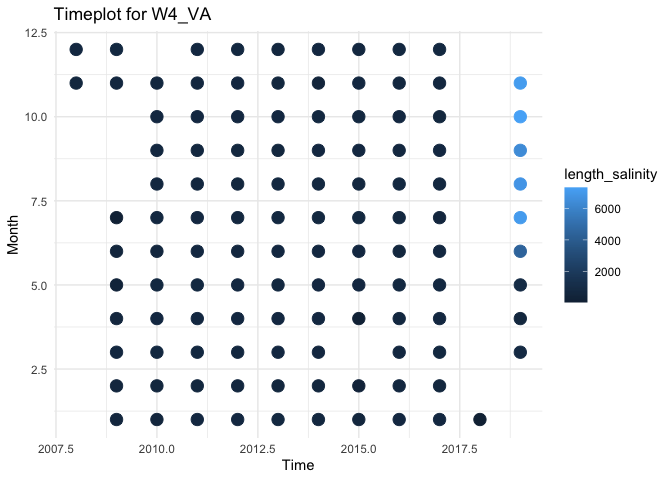
\includegraphics{DEBY_raw_env_files/figure-latex/timeplot-1.pdf}

\hypertarget{calculate-days-above-and-below-thresholds-and-plot}{%
\section{Calculate days above and below thresholds and
plot}\label{calculate-days-above-and-below-thresholds-and-plot}}

\begin{Shaded}
\begin{Highlighting}[]
\CommentTok{\# open up a blank data frame that spans all 12 months for all years of data collection for this site}
\CommentTok{\# we will merge this with the observations so that we can plot over time }

\NormalTok{complete\_year\_month }\OtherTok{\textless{}{-}} \FunctionTok{expand.grid}\NormalTok{(}
  \AttributeTok{year =} \FunctionTok{unique}\NormalTok{(firstyear}\SpecialCharTok{:}\NormalTok{finalyear),}
  \AttributeTok{month =} \DecValTok{1}\SpecialCharTok{:}\DecValTok{12}
\NormalTok{)}
\end{Highlighting}
\end{Shaded}

\hypertarget{start-with-low-salinity-stress}{%
\section{start with low salinity
stress}\label{start-with-low-salinity-stress}}

\begin{Shaded}
\begin{Highlighting}[]
\CommentTok{\# first calculate for low salinity}
\NormalTok{S2\_DEBY}\SpecialCharTok{$}\NormalTok{low\_sal\_stress }\OtherTok{\textless{}{-}}\NormalTok{ S2\_DEBY}\SpecialCharTok{$}\NormalTok{salinity }\SpecialCharTok{\textless{}} \DecValTok{12}

\NormalTok{low\_sal\_stress\_count }\OtherTok{\textless{}{-}}\NormalTok{ S2\_DEBY }\SpecialCharTok{\%\textgreater{}\%}
  \FunctionTok{mutate}\NormalTok{(}\AttributeTok{year =} \FunctionTok{year}\NormalTok{(datetime), }
         \AttributeTok{month =} \FunctionTok{month}\NormalTok{(datetime), }
         \AttributeTok{day =} \FunctionTok{day}\NormalTok{(datetime)) }\SpecialCharTok{\%\textgreater{}\%} 
  \FunctionTok{filter}\NormalTok{(low\_sal\_stress }\SpecialCharTok{==} \DecValTok{1}\NormalTok{) }\SpecialCharTok{\%\textgreater{}\%}  
  \FunctionTok{distinct}\NormalTok{(year, month, day) }\SpecialCharTok{\%\textgreater{}\%}  \CommentTok{\# remove dups}
  \FunctionTok{group\_by}\NormalTok{(year, month) }\SpecialCharTok{\%\textgreater{}\%}
  \FunctionTok{summarise}\NormalTok{(}\AttributeTok{low\_sal\_stress =} \FunctionTok{n}\NormalTok{(), }\AttributeTok{.groups =} \StringTok{"drop"}\NormalTok{) }\CommentTok{\# group all occurrences together by month rather than by numeric day}

\FunctionTok{print}\NormalTok{(low\_sal\_stress\_count)}
\end{Highlighting}
\end{Shaded}

\begin{verbatim}
## # A tibble: 20 x 3
##     year month low_sal_stress
##    <dbl> <dbl>          <int>
##  1  2003     6              3
##  2  2004     9              4
##  3  2005     4              7
##  4  2007     1              1
##  5  2009    12              1
##  6  2010     2              1
##  7  2010     4              3
##  8  2011     9              1
##  9  2014     5              7
## 10  2018     5              1
## 11  2018     6              7
## 12  2018     7              5
## 13  2018    10              5
## 14  2018    11             12
## 15  2018    12             11
## 16  2019     1             21
## 17  2019     2              7
## 18  2019     3             24
## 19  2019     4              4
## 20  2020    12              1
\end{verbatim}

\begin{Shaded}
\begin{Highlighting}[]
\CommentTok{\# this plots low sal stress days only, years with no observations of low salinity stress will not appear in the graph }
\FunctionTok{ggplot}\NormalTok{(low\_sal\_stress\_count, }\FunctionTok{aes}\NormalTok{(}\AttributeTok{x =} \FunctionTok{factor}\NormalTok{(month), }\AttributeTok{y =}\NormalTok{ low\_sal\_stress, }\AttributeTok{fill =} \FunctionTok{factor}\NormalTok{(month))) }\SpecialCharTok{+}
  \FunctionTok{geom\_bar}\NormalTok{(}\AttributeTok{stat =} \StringTok{"identity"}\NormalTok{, }\AttributeTok{fill =} \StringTok{"\#1f77b4"}\NormalTok{) }\SpecialCharTok{+}
  \FunctionTok{facet\_wrap}\NormalTok{(}\SpecialCharTok{\textasciitilde{}}\NormalTok{ year) }\SpecialCharTok{+}
  \FunctionTok{labs}\NormalTok{(}\AttributeTok{title =} \StringTok{"S2\_DEBY: count of low salinity (\textless{} 12 ppt) days per month"}\NormalTok{,}
       \AttributeTok{x =} \StringTok{"month"}\NormalTok{,}
       \AttributeTok{y =} \StringTok{"count of days"}\NormalTok{) }\SpecialCharTok{+}
  \FunctionTok{theme\_minimal}\NormalTok{()}
\end{Highlighting}
\end{Shaded}

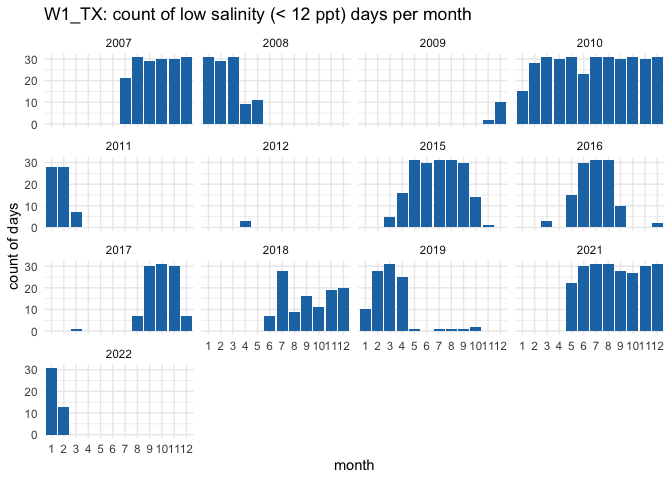
\includegraphics{DEBY_raw_env_files/figure-latex/low-sal-stress-1.pdf}

\begin{Shaded}
\begin{Highlighting}[]
\CommentTok{\# Merge with the original dataset, filling missing values with 0 for low\_sal\_stress}
\NormalTok{low\_sal\_complete\_data }\OtherTok{\textless{}{-}}\NormalTok{ complete\_year\_month }\SpecialCharTok{\%\textgreater{}\%}
  \FunctionTok{left\_join}\NormalTok{(low\_sal\_stress\_count, }\AttributeTok{by =} \FunctionTok{c}\NormalTok{(}\StringTok{"year"}\NormalTok{, }\StringTok{"month"}\NormalTok{)) }\SpecialCharTok{\%\textgreater{}\%}
  \FunctionTok{mutate}\NormalTok{(}\AttributeTok{low\_sal\_stress =} \FunctionTok{ifelse}\NormalTok{(}\FunctionTok{is.na}\NormalTok{(low\_sal\_stress), }\DecValTok{0}\NormalTok{, low\_sal\_stress))}

\NormalTok{low\_sal\_complete\_data}\SpecialCharTok{$}\NormalTok{month }\OtherTok{\textless{}{-}} \FunctionTok{as.numeric}\NormalTok{(low\_sal\_complete\_data}\SpecialCharTok{$}\NormalTok{month)}

\CommentTok{\# bars}
\FunctionTok{ggplot}\NormalTok{(low\_sal\_complete\_data, }\FunctionTok{aes}\NormalTok{(}\AttributeTok{x =} \FunctionTok{factor}\NormalTok{(month), }\AttributeTok{y =}\NormalTok{ low\_sal\_stress)) }\SpecialCharTok{+}
  \FunctionTok{geom\_bar}\NormalTok{(}\AttributeTok{stat =} \StringTok{"identity"}\NormalTok{, }\AttributeTok{fill =} \StringTok{"\#1f77b4"}\NormalTok{) }\SpecialCharTok{+} 
  \FunctionTok{facet\_wrap}\NormalTok{(}\SpecialCharTok{\textasciitilde{}}\NormalTok{ year) }\SpecialCharTok{+}
  \FunctionTok{labs}\NormalTok{(}\AttributeTok{title =} \StringTok{"S2\_DEBY: count of low salinity (\textless{} 12 ppt) days per month"}\NormalTok{,}
       \AttributeTok{x =} \StringTok{"month"}\NormalTok{,}
       \AttributeTok{y =} \StringTok{"count of low salinity stress days"}\NormalTok{) }\SpecialCharTok{+}
  \FunctionTok{theme\_minimal}\NormalTok{()}
\end{Highlighting}
\end{Shaded}

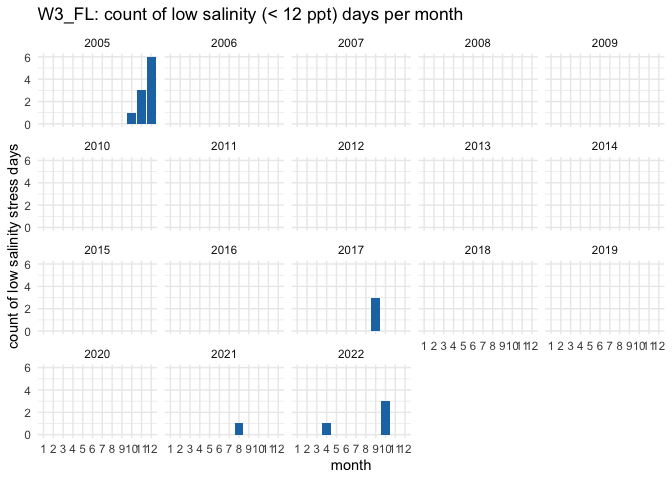
\includegraphics{DEBY_raw_env_files/figure-latex/low-sal-stress-2.pdf}

\begin{Shaded}
\begin{Highlighting}[]
\CommentTok{\# points}
\FunctionTok{ggplot}\NormalTok{(low\_sal\_complete\_data, }\FunctionTok{aes}\NormalTok{(}\AttributeTok{x =} \FunctionTok{factor}\NormalTok{(month), }\AttributeTok{y =}\NormalTok{ low\_sal\_stress)) }\SpecialCharTok{+}
  \FunctionTok{geom\_point}\NormalTok{(}\AttributeTok{color =} \StringTok{"\#1f77b4"}\NormalTok{, }\AttributeTok{size =} \DecValTok{2}\NormalTok{) }\SpecialCharTok{+} 
  \FunctionTok{facet\_wrap}\NormalTok{(}\SpecialCharTok{\textasciitilde{}}\NormalTok{ year) }\SpecialCharTok{+}  
  \FunctionTok{labs}\NormalTok{(}\AttributeTok{title =} \StringTok{"S2\_DEBY: count of low salinity (\textless{} 12 ppt) days per month"}\NormalTok{,}
       \AttributeTok{x =} \StringTok{"month"}\NormalTok{,}
       \AttributeTok{y =} \StringTok{"count of low salinity stress days"}\NormalTok{) }\SpecialCharTok{+}
  \FunctionTok{theme\_minimal}\NormalTok{()}
\end{Highlighting}
\end{Shaded}

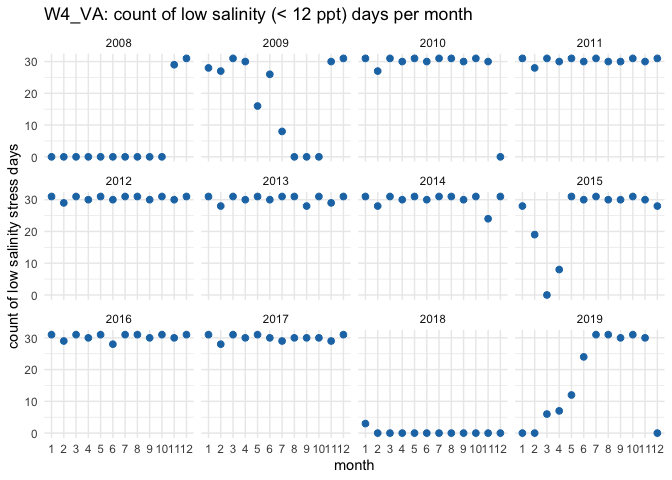
\includegraphics{DEBY_raw_env_files/figure-latex/low-sal-stress-3.pdf}

\hypertarget{now-calculate-for-high-salinity-stress}{%
\section{now calculate for high salinity
stress}\label{now-calculate-for-high-salinity-stress}}

\begin{Shaded}
\begin{Highlighting}[]
\NormalTok{S2\_DEBY}\SpecialCharTok{$}\NormalTok{high\_sal\_stress }\OtherTok{\textless{}{-}}\NormalTok{ S2\_DEBY}\SpecialCharTok{$}\NormalTok{salinity }\SpecialCharTok{\textgreater{}} \DecValTok{35}

\NormalTok{high\_sal\_stress\_count }\OtherTok{\textless{}{-}}\NormalTok{ S2\_DEBY }\SpecialCharTok{\%\textgreater{}\%}
  \FunctionTok{mutate}\NormalTok{(}\AttributeTok{year =} \FunctionTok{year}\NormalTok{(datetime), }
         \AttributeTok{month =} \FunctionTok{month}\NormalTok{(datetime), }
         \AttributeTok{day =} \FunctionTok{day}\NormalTok{(datetime)) }\SpecialCharTok{\%\textgreater{}\%} 
  \FunctionTok{filter}\NormalTok{(high\_sal\_stress }\SpecialCharTok{==} \DecValTok{1}\NormalTok{) }\SpecialCharTok{\%\textgreater{}\%}  
  \FunctionTok{distinct}\NormalTok{(year, month, day) }\SpecialCharTok{\%\textgreater{}\%}  \CommentTok{\# remove dups}
  \FunctionTok{group\_by}\NormalTok{(year, month) }\SpecialCharTok{\%\textgreater{}\%}
  \FunctionTok{summarise}\NormalTok{(}\AttributeTok{high\_sal\_stress =} \FunctionTok{n}\NormalTok{(), }\AttributeTok{.groups =} \StringTok{"drop"}\NormalTok{) }\CommentTok{\# group all occurrences together by month rather than by numeric day}

\FunctionTok{print}\NormalTok{(high\_sal\_stress\_count) }\CommentTok{\# 0 high sal stress days}
\end{Highlighting}
\end{Shaded}

\begin{verbatim}
## # A tibble: 0 x 3
## # i 3 variables: year <dbl>, month <dbl>, high_sal_stress <int>
\end{verbatim}

\hypertarget{high-temp-stress-calculations}{%
\section{high temp stress
calculations}\label{high-temp-stress-calculations}}

\begin{Shaded}
\begin{Highlighting}[]
\NormalTok{S2\_DEBY}\SpecialCharTok{$}\NormalTok{high\_temp\_stress }\OtherTok{\textless{}{-}}\NormalTok{ S2\_DEBY}\SpecialCharTok{$}\NormalTok{temp }\SpecialCharTok{\textgreater{}} \DecValTok{28}

\NormalTok{high\_temp\_stress\_count }\OtherTok{\textless{}{-}}\NormalTok{ S2\_DEBY }\SpecialCharTok{\%\textgreater{}\%}
  \FunctionTok{mutate}\NormalTok{(}\AttributeTok{year =} \FunctionTok{year}\NormalTok{(datetime), }
         \AttributeTok{month =} \FunctionTok{month}\NormalTok{(datetime), }
         \AttributeTok{day =} \FunctionTok{day}\NormalTok{(datetime)) }\SpecialCharTok{\%\textgreater{}\%} 
  \FunctionTok{filter}\NormalTok{(high\_temp\_stress }\SpecialCharTok{==} \DecValTok{1}\NormalTok{) }\SpecialCharTok{\%\textgreater{}\%}  
  \FunctionTok{distinct}\NormalTok{(year, month, day) }\SpecialCharTok{\%\textgreater{}\%}  \CommentTok{\# remove dups}
  \FunctionTok{group\_by}\NormalTok{(year, month) }\SpecialCharTok{\%\textgreater{}\%}
  \FunctionTok{summarise}\NormalTok{(}\AttributeTok{high\_temp\_stress =} \FunctionTok{n}\NormalTok{(), }\AttributeTok{.groups =} \StringTok{"drop"}\NormalTok{) }\CommentTok{\# group all occurrences together by month rather than by numeric day}

\FunctionTok{print}\NormalTok{(high\_temp\_stress\_count)}
\end{Highlighting}
\end{Shaded}

\begin{verbatim}
## # A tibble: 73 x 3
##     year month high_temp_stress
##    <dbl> <dbl>            <int>
##  1  2003     6                2
##  2  2003     7               16
##  3  2003     8               17
##  4  2004     6                1
##  5  2004     7               26
##  6  2004     8                8
##  7  2004     9                1
##  8  2005     7               26
##  9  2005     8               18
## 10  2005     9                7
## # i 63 more rows
\end{verbatim}

\begin{Shaded}
\begin{Highlighting}[]
\FunctionTok{ggplot}\NormalTok{(high\_temp\_stress\_count, }\FunctionTok{aes}\NormalTok{(}\AttributeTok{x =} \FunctionTok{factor}\NormalTok{(month), }\AttributeTok{y =}\NormalTok{ high\_temp\_stress, }\AttributeTok{fill =} \FunctionTok{factor}\NormalTok{(month))) }\SpecialCharTok{+}
  \FunctionTok{geom\_bar}\NormalTok{(}\AttributeTok{stat =} \StringTok{"identity"}\NormalTok{, }\AttributeTok{fill =} \StringTok{"\#DD4124FF"}\NormalTok{) }\SpecialCharTok{+}
  \FunctionTok{facet\_wrap}\NormalTok{(}\SpecialCharTok{\textasciitilde{}}\NormalTok{ year) }\SpecialCharTok{+}
  \FunctionTok{labs}\NormalTok{(}\AttributeTok{title =} \StringTok{"S2\_DEBY: count of high temperature (\textgreater{} 28 C) days per month"}\NormalTok{,}
       \AttributeTok{x =} \StringTok{"month"}\NormalTok{,}
       \AttributeTok{y =} \StringTok{"count of days"}\NormalTok{) }\SpecialCharTok{+}
  \FunctionTok{theme\_minimal}\NormalTok{()}
\end{Highlighting}
\end{Shaded}

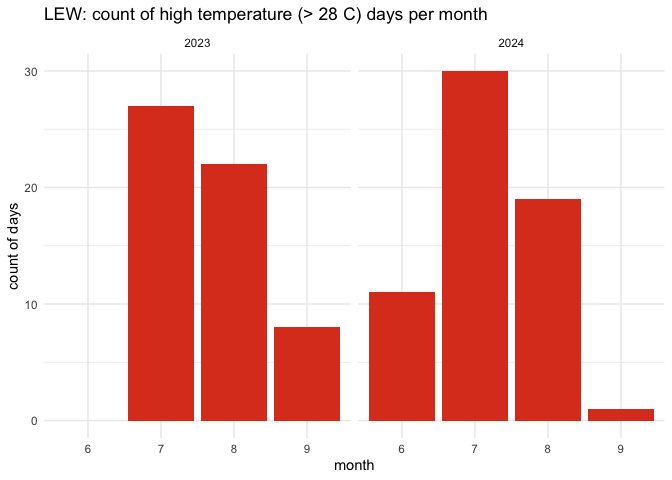
\includegraphics{DEBY_raw_env_files/figure-latex/high-temp-stress-1.pdf}

\begin{Shaded}
\begin{Highlighting}[]
\NormalTok{high\_temp\_complete\_data }\OtherTok{\textless{}{-}}\NormalTok{ complete\_year\_month }\SpecialCharTok{\%\textgreater{}\%}
  \FunctionTok{left\_join}\NormalTok{(high\_temp\_stress\_count, }\AttributeTok{by =} \FunctionTok{c}\NormalTok{(}\StringTok{"year"}\NormalTok{, }\StringTok{"month"}\NormalTok{)) }\SpecialCharTok{\%\textgreater{}\%}
  \FunctionTok{mutate}\NormalTok{(}\AttributeTok{high\_temp\_stress =} \FunctionTok{ifelse}\NormalTok{(}\FunctionTok{is.na}\NormalTok{(high\_temp\_stress), }\DecValTok{0}\NormalTok{, high\_temp\_stress))}

\NormalTok{high\_temp\_complete\_data}\SpecialCharTok{$}\NormalTok{month }\OtherTok{\textless{}{-}} \FunctionTok{as.numeric}\NormalTok{(high\_temp\_complete\_data}\SpecialCharTok{$}\NormalTok{month)}

\CommentTok{\# bars}
\FunctionTok{ggplot}\NormalTok{(high\_temp\_complete\_data, }\FunctionTok{aes}\NormalTok{(}\AttributeTok{x =} \FunctionTok{factor}\NormalTok{(month), }\AttributeTok{y =}\NormalTok{ high\_temp\_stress)) }\SpecialCharTok{+}
  \FunctionTok{geom\_bar}\NormalTok{(}\AttributeTok{stat =} \StringTok{"identity"}\NormalTok{, }\AttributeTok{fill =} \StringTok{"\#DD4124FF"}\NormalTok{) }\SpecialCharTok{+} 
  \FunctionTok{facet\_wrap}\NormalTok{(}\SpecialCharTok{\textasciitilde{}}\NormalTok{ year) }\SpecialCharTok{+}
  \FunctionTok{labs}\NormalTok{(}\AttributeTok{title =} \StringTok{"S2\_DEBY: count of high temperature (\textgreater{} 28 C) days per month"}\NormalTok{,}
       \AttributeTok{x =} \StringTok{"month"}\NormalTok{,}
       \AttributeTok{y =} \StringTok{"count of days"}\NormalTok{) }\SpecialCharTok{+}
  \FunctionTok{theme\_minimal}\NormalTok{()}
\end{Highlighting}
\end{Shaded}

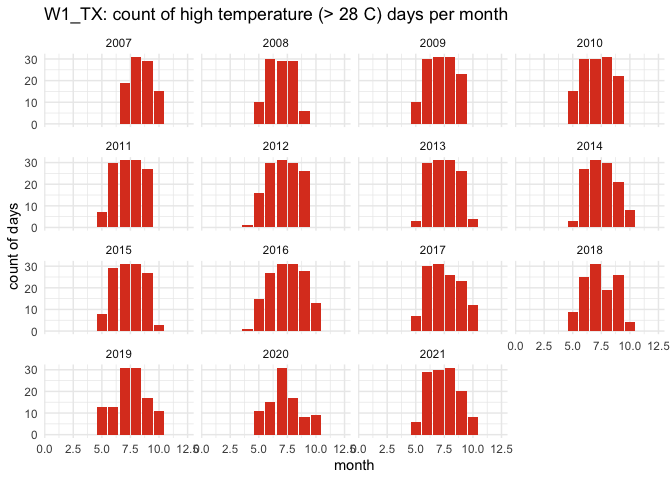
\includegraphics{DEBY_raw_env_files/figure-latex/high-temp-stress-2.pdf}

\begin{Shaded}
\begin{Highlighting}[]
\CommentTok{\# points}
\FunctionTok{ggplot}\NormalTok{(high\_temp\_complete\_data, }\FunctionTok{aes}\NormalTok{(}\AttributeTok{x =} \FunctionTok{factor}\NormalTok{(month), }\AttributeTok{y =}\NormalTok{ high\_temp\_stress)) }\SpecialCharTok{+}
  \FunctionTok{geom\_point}\NormalTok{(}\AttributeTok{color =} \StringTok{"\#DD4124FF"}\NormalTok{, }\AttributeTok{size =} \DecValTok{2}\NormalTok{) }\SpecialCharTok{+} 
  \FunctionTok{facet\_wrap}\NormalTok{(}\SpecialCharTok{\textasciitilde{}}\NormalTok{ year) }\SpecialCharTok{+}  
  \FunctionTok{labs}\NormalTok{(}\AttributeTok{title =} \StringTok{"S2\_DEBY: count of high temperature (\textgreater{} 28 C) days per month"}\NormalTok{,}
       \AttributeTok{x =} \StringTok{"month"}\NormalTok{,}
       \AttributeTok{y =} \StringTok{"count of days"}\NormalTok{) }\SpecialCharTok{+}
  \FunctionTok{theme\_minimal}\NormalTok{()}
\end{Highlighting}
\end{Shaded}

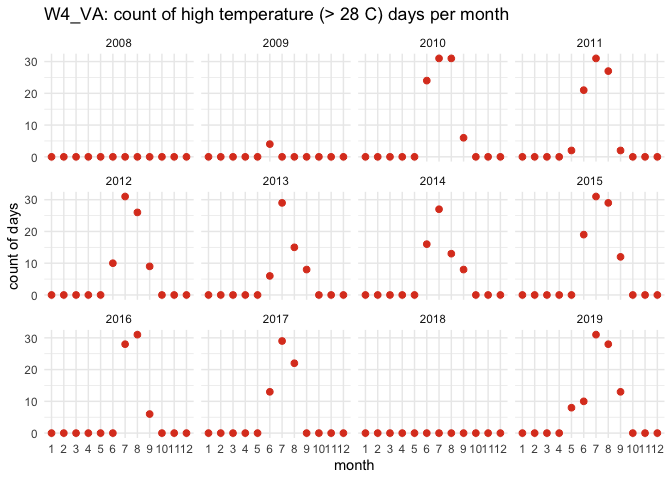
\includegraphics{DEBY_raw_env_files/figure-latex/high-temp-stress-3.pdf}

\hypertarget{we-can-now-calculate-a-list-of-variables-that-we-will-have-collected-for-all-sites.-this-will-allow-us-to-compare-sites-easily.-we-will-calculate-the-number-of-observations-from-each-site-the-mean-annual-maximum-annual-and-minimum-annual-value-for-all-variables.}{%
\subsubsection{We can now calculate a list of variables that we will
have collected for all sites. This will allow us to compare sites
easily. We will calculate the number of observations from each site, the
mean annual, maximum annual, and minimum annual value for all
variables.}\label{we-can-now-calculate-a-list-of-variables-that-we-will-have-collected-for-all-sites.-this-will-allow-us-to-compare-sites-easily.-we-will-calculate-the-number-of-observations-from-each-site-the-mean-annual-maximum-annual-and-minimum-annual-value-for-all-variables.}}

Our list of variables includes:

\begin{itemize}
\item
  Mean\_Annual\_Temperature\_C: average of all available data
\item
  Mean\_max\_temperature\_C: average of maximums for each year
\item
  Mean\_min\_temperature\_C: average of minimums for each year
\item
  Temperature\_st\_dev: standard deviation of all available data
\item
  Temperature\_n: total number of data points
\item
  Temperature\_years: number of years in data set
\item
  Mean\_Annual\_Salinity\_ppt: average of all available data
\item
  Mean\_min\_Salinity\_ppt: average of minimums for each year
\item
  Mean\_max\_Salinity\_ppt: average of maximums for each year
\item
  Salinity\_st\_dev: standard deviation of all available data
\item
  Salinity\_n: total number of data points
\item
  Salinity\_years: number of years in data set
\end{itemize}

\begin{Shaded}
\begin{Highlighting}[]
\CommentTok{\#Calculate temperature variables. }
\NormalTok{Mean\_Annual\_Temperature\_C }\OtherTok{\textless{}{-}} \FunctionTok{mean}\NormalTok{(S2\_DEBY}\SpecialCharTok{$}\NormalTok{temp)}
\NormalTok{Mean\_max\_temperature\_C }\OtherTok{\textless{}{-}} \FunctionTok{mean}\NormalTok{(S2\_DEBY\_envryear}\SpecialCharTok{$}\NormalTok{max\_temp)}
\NormalTok{Mean\_min\_temperature\_C }\OtherTok{\textless{}{-}} \FunctionTok{mean}\NormalTok{(S2\_DEBY\_envryear}\SpecialCharTok{$}\NormalTok{min\_temp)}
\NormalTok{Temperature\_st\_dev }\OtherTok{\textless{}{-}} \FunctionTok{sd}\NormalTok{(S2\_DEBY}\SpecialCharTok{$}\NormalTok{temp)}
\NormalTok{Temperature\_n }\OtherTok{\textless{}{-}} \FunctionTok{nrow}\NormalTok{(S2\_DEBY)}
\NormalTok{Temperature\_years }\OtherTok{\textless{}{-}} \FunctionTok{nrow}\NormalTok{(S2\_DEBY\_envryear)}
\NormalTok{high\_temp\_stress\_days }\OtherTok{\textless{}{-}} \FunctionTok{sum}\NormalTok{(high\_temp\_stress\_count}\SpecialCharTok{$}\NormalTok{high\_temp\_stress)}
\NormalTok{frac\_high\_temp\_stress\_days }\OtherTok{\textless{}{-}}\NormalTok{ high\_temp\_stress\_days}\SpecialCharTok{/}\FunctionTok{nrow}\NormalTok{(S2\_DEBY\_envrday)}

\NormalTok{Mean\_Monthly\_Temperature\_C }\OtherTok{\textless{}{-}}\NormalTok{ S2\_DEBY\_envrmonth }\SpecialCharTok{\%\textgreater{}\%}
  \FunctionTok{filter}\NormalTok{(}\SpecialCharTok{!}\FunctionTok{is.na}\NormalTok{(month)) }\SpecialCharTok{\%\textgreater{}\%} 
  \FunctionTok{group\_by}\NormalTok{(month) }\SpecialCharTok{\%\textgreater{}\%}
  \FunctionTok{summarise}\NormalTok{(}\AttributeTok{Mean\_Temperature =} \FunctionTok{mean}\NormalTok{(mean\_temp))}

\NormalTok{Mean\_min\_Monthly\_Temperature\_C }\OtherTok{\textless{}{-}}\NormalTok{ S2\_DEBY\_envrmonth }\SpecialCharTok{\%\textgreater{}\%}
  \FunctionTok{filter}\NormalTok{(}\SpecialCharTok{!}\FunctionTok{is.na}\NormalTok{(month)) }\SpecialCharTok{\%\textgreater{}\%} 
  \FunctionTok{group\_by}\NormalTok{(month) }\SpecialCharTok{\%\textgreater{}\%}
  \FunctionTok{summarise}\NormalTok{(}\AttributeTok{Mean\_min\_Temperature =} \FunctionTok{mean}\NormalTok{(min\_temp))}

\NormalTok{Mean\_max\_Monthly\_Temperature\_C }\OtherTok{\textless{}{-}}\NormalTok{ S2\_DEBY\_envrmonth }\SpecialCharTok{\%\textgreater{}\%}
  \FunctionTok{filter}\NormalTok{(}\SpecialCharTok{!}\FunctionTok{is.na}\NormalTok{(month)) }\SpecialCharTok{\%\textgreater{}\%} 
  \FunctionTok{group\_by}\NormalTok{(month) }\SpecialCharTok{\%\textgreater{}\%}
  \FunctionTok{summarise}\NormalTok{(}\AttributeTok{Mean\_max\_Temperature =} \FunctionTok{mean}\NormalTok{(max\_temp))}

\CommentTok{\#Create a data frame to store the temperature results}
\NormalTok{S2\_DEBY\_temp }\OtherTok{\textless{}{-}} \FunctionTok{cbind}\NormalTok{(site\_name, download\_date, source\_description, lat, lon, firstyear, finalyear, Mean\_Annual\_Temperature\_C, Mean\_max\_temperature\_C, Mean\_min\_temperature\_C, Temperature\_st\_dev, high\_temp\_stress\_days, frac\_high\_temp\_stress\_days, Temperature\_n, Temperature\_years, collection\_type)}
\FunctionTok{print}\NormalTok{(S2\_DEBY\_temp)}
\end{Highlighting}
\end{Shaded}

\begin{verbatim}
##      site_name download_date
## [1,] "DEBY"    "04-02-2024" 
##      source_description                                      lat        
## [1,] "Virginia Estuarine and Coastal Observing System, VIMS" "37.247284"
##      lon          firstyear finalyear Mean_Annual_Temperature_C
## [1,] "-76.499369" "2003"    "2024"    "17.1242424156129"       
##      Mean_max_temperature_C Mean_min_temperature_C Temperature_st_dev
## [1,] "30.1437727272727"     "3.54609090909091"     "8.07505645766884"
##      high_temp_stress_days frac_high_temp_stress_days Temperature_n
## [1,] "999"                 "0.141121627348496"        "667193"     
##      Temperature_years collection_type
## [1,] "22"              "continuous"
\end{verbatim}

\begin{Shaded}
\begin{Highlighting}[]
\NormalTok{S2\_DEBY\_monthly\_temp }\OtherTok{\textless{}{-}} \FunctionTok{cbind}\NormalTok{(Mean\_Monthly\_Temperature\_C, Mean\_min\_Monthly\_Temperature\_C, Mean\_max\_Monthly\_Temperature\_C)}
\NormalTok{S2\_DEBY\_monthly\_temp }\OtherTok{\textless{}{-}}\NormalTok{ S2\_DEBY\_monthly\_temp[, }\SpecialCharTok{!}\FunctionTok{duplicated}\NormalTok{(}\FunctionTok{names}\NormalTok{(S2\_DEBY\_monthly\_temp))]}
\FunctionTok{print}\NormalTok{(S2\_DEBY\_monthly\_temp)}
\end{Highlighting}
\end{Shaded}

\begin{verbatim}
##    month Mean_Temperature Mean_min_Temperature Mean_max_Temperature
## 1      1         6.248902             3.509158             9.135947
## 2      2         5.881779             3.799700             8.673250
## 3      3         9.237711             5.800350            13.624800
## 4      4        14.309465            10.409050            19.282150
## 5      5        19.689801            15.947429            24.766905
## 6      6        24.540921            20.894762            28.528952
## 7      7        27.515154            25.081381            30.621190
## 8      8        27.675389            25.426048            30.577762
## 9      9        25.214310            22.079905            28.680190
## 10    10        20.113651            15.810810            24.171571
## 11    11        13.792849             9.980619            18.055333
## 12    12         9.120592             6.525900            12.196900
\end{verbatim}

\begin{Shaded}
\begin{Highlighting}[]
\CommentTok{\# Write to the combined file with all sites }
\FunctionTok{write.table}\NormalTok{(S2\_DEBY\_temp, }\StringTok{"/Users/madelineeppley/GitHub/MVP{-}H2F{-}HatcheryField/data/environment/all\_temperature.csv"}\NormalTok{, }\AttributeTok{sep =} \StringTok{","}\NormalTok{, }\AttributeTok{append =} \ConstantTok{TRUE}\NormalTok{, }\AttributeTok{col.names =} \ConstantTok{FALSE}\NormalTok{, }\AttributeTok{row.names =} \ConstantTok{FALSE}\NormalTok{) }\CommentTok{\# The column names should be changed to FALSE after 1st row is added to the data frame}

\CommentTok{\# Write to a unique new CSV file}
\FunctionTok{write.csv}\NormalTok{(S2\_DEBY\_temp, }\StringTok{"/Users/madelineeppley/GitHub/MVP{-}H2F{-}HatcheryField/data/environment/S2\_DEBY\_temperature.csv"}\NormalTok{)}

\CommentTok{\# Write all montly data to a unique new CSV file}
\FunctionTok{write.csv}\NormalTok{(S2\_DEBY\_monthly\_temp, }\StringTok{"/Users/madelineeppley/GitHub/MVP{-}H2F{-}HatcheryField/data/environment/S2\_DEBY\_monthly\_temp.csv"}\NormalTok{)}
\end{Highlighting}
\end{Shaded}

\begin{Shaded}
\begin{Highlighting}[]
\CommentTok{\#Calculate the salinity variables}
\NormalTok{Mean\_Annual\_Salinity\_ppt }\OtherTok{\textless{}{-}} \FunctionTok{mean}\NormalTok{(S2\_DEBY}\SpecialCharTok{$}\NormalTok{salinity)}
\NormalTok{Mean\_max\_Salinity\_ppt }\OtherTok{\textless{}{-}} \FunctionTok{mean}\NormalTok{(S2\_DEBY\_envryear}\SpecialCharTok{$}\NormalTok{max\_salinity)}
\NormalTok{Mean\_min\_Salinity\_ppt }\OtherTok{\textless{}{-}} \FunctionTok{mean}\NormalTok{(S2\_DEBY\_envryear}\SpecialCharTok{$}\NormalTok{min\_salinity)}
\NormalTok{Salinity\_st\_dev }\OtherTok{\textless{}{-}} \FunctionTok{sd}\NormalTok{(S2\_DEBY}\SpecialCharTok{$}\NormalTok{salinity)}
\NormalTok{Salinity\_n }\OtherTok{\textless{}{-}} \FunctionTok{nrow}\NormalTok{(S2\_DEBY)}
\NormalTok{Salinity\_years }\OtherTok{\textless{}{-}} \FunctionTok{nrow}\NormalTok{(S2\_DEBY\_envryear)}
\NormalTok{high\_sal\_stress\_days }\OtherTok{\textless{}{-}} \FunctionTok{sum}\NormalTok{(high\_sal\_stress\_count}\SpecialCharTok{$}\NormalTok{high\_sal\_stress)}
\NormalTok{low\_sal\_stress\_days }\OtherTok{\textless{}{-}} \FunctionTok{sum}\NormalTok{(low\_sal\_stress\_count}\SpecialCharTok{$}\NormalTok{low\_sal\_stress)}
\NormalTok{frac\_high\_sal\_stress\_days }\OtherTok{\textless{}{-}}\NormalTok{ high\_sal\_stress\_days}\SpecialCharTok{/}\FunctionTok{nrow}\NormalTok{(S2\_DEBY\_envrday)}
\NormalTok{frac\_low\_sal\_stress\_days }\OtherTok{\textless{}{-}}\NormalTok{ low\_sal\_stress\_days}\SpecialCharTok{/}\FunctionTok{nrow}\NormalTok{(S2\_DEBY\_envrday)}

\NormalTok{Mean\_Monthly\_Salinity }\OtherTok{\textless{}{-}}\NormalTok{ S2\_DEBY\_envrmonth }\SpecialCharTok{\%\textgreater{}\%}
  \FunctionTok{filter}\NormalTok{(}\SpecialCharTok{!}\FunctionTok{is.na}\NormalTok{(month)) }\SpecialCharTok{\%\textgreater{}\%}
  \FunctionTok{group\_by}\NormalTok{(month) }\SpecialCharTok{\%\textgreater{}\%}
  \FunctionTok{summarise}\NormalTok{(}\AttributeTok{Mean\_Salinity =} \FunctionTok{mean}\NormalTok{(mean\_salinity))}

\NormalTok{Min\_Monthly\_Salinity }\OtherTok{\textless{}{-}}\NormalTok{ S2\_DEBY\_envrmonth }\SpecialCharTok{\%\textgreater{}\%}
  \FunctionTok{filter}\NormalTok{(}\SpecialCharTok{!}\FunctionTok{is.na}\NormalTok{(month)) }\SpecialCharTok{\%\textgreater{}\%}
  \FunctionTok{group\_by}\NormalTok{(month) }\SpecialCharTok{\%\textgreater{}\%}
  \FunctionTok{summarise}\NormalTok{(}\AttributeTok{Min\_Salinity =} \FunctionTok{mean}\NormalTok{(min\_salinity))}

\NormalTok{Max\_Monthly\_Salinity }\OtherTok{\textless{}{-}}\NormalTok{ S2\_DEBY\_envrmonth }\SpecialCharTok{\%\textgreater{}\%}
  \FunctionTok{filter}\NormalTok{(}\SpecialCharTok{!}\FunctionTok{is.na}\NormalTok{(month)) }\SpecialCharTok{\%\textgreater{}\%}
  \FunctionTok{group\_by}\NormalTok{(month) }\SpecialCharTok{\%\textgreater{}\%}
  \FunctionTok{summarise}\NormalTok{(}\AttributeTok{Max\_Salinity =} \FunctionTok{mean}\NormalTok{(max\_salinity))}

\CommentTok{\#Create a data frame to store the temperature results}
\NormalTok{S2\_DEBY\_salinity }\OtherTok{\textless{}{-}} \FunctionTok{cbind}\NormalTok{(site\_name, download\_date, source\_description, lat, lon, firstyear, finalyear, Mean\_Annual\_Salinity\_ppt, Mean\_max\_Salinity\_ppt, Mean\_min\_Salinity\_ppt, high\_sal\_stress\_days,low\_sal\_stress\_days, frac\_high\_sal\_stress\_days, frac\_low\_sal\_stress\_days, Salinity\_st\_dev, Salinity\_n, Salinity\_years, collection\_type)}
\FunctionTok{print}\NormalTok{(S2\_DEBY\_salinity)}
\end{Highlighting}
\end{Shaded}

\begin{verbatim}
##      site_name download_date
## [1,] "DEBY"    "04-02-2024" 
##      source_description                                      lat        
## [1,] "Virginia Estuarine and Coastal Observing System, VIMS" "37.247284"
##      lon          firstyear finalyear Mean_Annual_Salinity_ppt
## [1,] "-76.499369" "2003"    "2024"    "19.3391307162995"      
##      Mean_max_Salinity_ppt Mean_min_Salinity_ppt high_sal_stress_days
## [1,] "24.1890909090909"    "12.9063636363636"    "0"                 
##      low_sal_stress_days frac_high_sal_stress_days frac_low_sal_stress_days
## [1,] "126"               "0"                       "0.0177991241700805"    
##      Salinity_st_dev    Salinity_n Salinity_years collection_type
## [1,] "2.56014876611224" "667193"   "22"           "continuous"
\end{verbatim}

\begin{Shaded}
\begin{Highlighting}[]
\NormalTok{S2\_DEBY\_monthly\_sal }\OtherTok{\textless{}{-}} \FunctionTok{cbind}\NormalTok{(Mean\_Monthly\_Salinity, Min\_Monthly\_Salinity, Max\_Monthly\_Salinity)}
\NormalTok{S2\_DEBY\_monthly\_sal }\OtherTok{\textless{}{-}}\NormalTok{ S2\_DEBY\_monthly\_sal[, }\SpecialCharTok{!}\FunctionTok{duplicated}\NormalTok{(}\FunctionTok{names}\NormalTok{(S2\_DEBY\_monthly\_sal))]}
\FunctionTok{print}\NormalTok{(S2\_DEBY\_monthly\_sal)}
\end{Highlighting}
\end{Shaded}

\begin{verbatim}
##    month Mean_Salinity Min_Salinity Max_Salinity
## 1      1      19.56410     17.08737     21.97211
## 2      2      18.76076     16.50700     21.34700
## 3      3      18.36119     15.51150     21.26900
## 4      4      17.80045     15.08300     20.35200
## 5      5      17.30105     14.86667     19.72571
## 6      6      17.99405     15.58762     20.85095
## 7      7      19.71824     17.06429     22.32476
## 8      8      20.54352     18.25524     22.71667
## 9      9      20.33304     18.54000     22.48571
## 10    10      20.33898     18.24048     22.49095
## 11    11      20.38709     17.95476     22.46286
## 12    12      20.00368     17.53350     22.10150
\end{verbatim}

\begin{Shaded}
\begin{Highlighting}[]
\CommentTok{\# Write to the combined file with all sites }
\FunctionTok{write.table}\NormalTok{(S2\_DEBY\_salinity, }\StringTok{"/Users/madelineeppley/GitHub/MVP{-}H2F{-}HatcheryField/data/environment/all\_salinity.csv"}\NormalTok{, }\AttributeTok{sep =} \StringTok{","}\NormalTok{, }\AttributeTok{append =} \ConstantTok{TRUE}\NormalTok{, }\AttributeTok{col.names =} \ConstantTok{FALSE}\NormalTok{, }\AttributeTok{row.names =} \ConstantTok{FALSE}\NormalTok{) }\CommentTok{\# The column names should be changed to FALSE after 1st row is added to the data frame}

\CommentTok{\# Write all year data to a unique new CSV file}
\FunctionTok{write.csv}\NormalTok{(S2\_DEBY\_salinity, }\StringTok{"/Users/madelineeppley/GitHub/MVP{-}H2F{-}HatcheryField/data/environment/S2\_DEBY\_salinity.csv"}\NormalTok{)}
\CommentTok{\# Write all montly data to a unique new CSV file}
\FunctionTok{write.csv}\NormalTok{(S2\_DEBY\_monthly\_sal, }\StringTok{"/Users/madelineeppley/GitHub/MVP{-}H2F{-}HatcheryField/data/environment/S2\_DEBY\_monthly\_sal.csv"}\NormalTok{)}
\end{Highlighting}
\end{Shaded}


\end{document}
